\chapter{Graphical Multivariate Representation}\label{appendix2}
\fixchapterheading

\vspace{0.8cm}

The graphical representation of relationships and functions involving more than a total of three variables is a difficult problem.  A function of two independent variables can be represented as a surface within a three-dimensional Cartesian coordinate system, but functions of more variables cannot be represented in this same fashion.  Chernoff (1973) invented a novel solution to this problem.  By assigning variables to different facial characteristics, Chernoff was able to uniquely represent up to 18 variables of data as a set of human faces.  Thus, an 18-dimensional data point can be represented in a single graphical image, allowing the analyst to perceive 18 characteristics simultaneously.  Chernoff's graphical technique was applied to the Utah parolee data in order to investigate whether recognizable patterns exist among recidivists relative to nonrecidivists.

From the Utah parolee data set, only 20 observations were selected for graphical representation.  Two subsets of the data were chosen to provide the greatest contrast between those who recidivated and those who did not.  From the set of 221 parolees that returned to prison, the BMA model was used to select the 10 parolees with the highest probability of returning to prison. Likewise, from the set of 285 parolees that did not return to prison, the 10 parolees with the lowest probability of returning to prison were selected for the other subset.  The faces were modeled using 15 different variables, where all of the most important predictors of recidivism were included.  The graphical representation of these 20 observations is presented in Figure B.1.

\begin{figure}[t]
\begin{center}
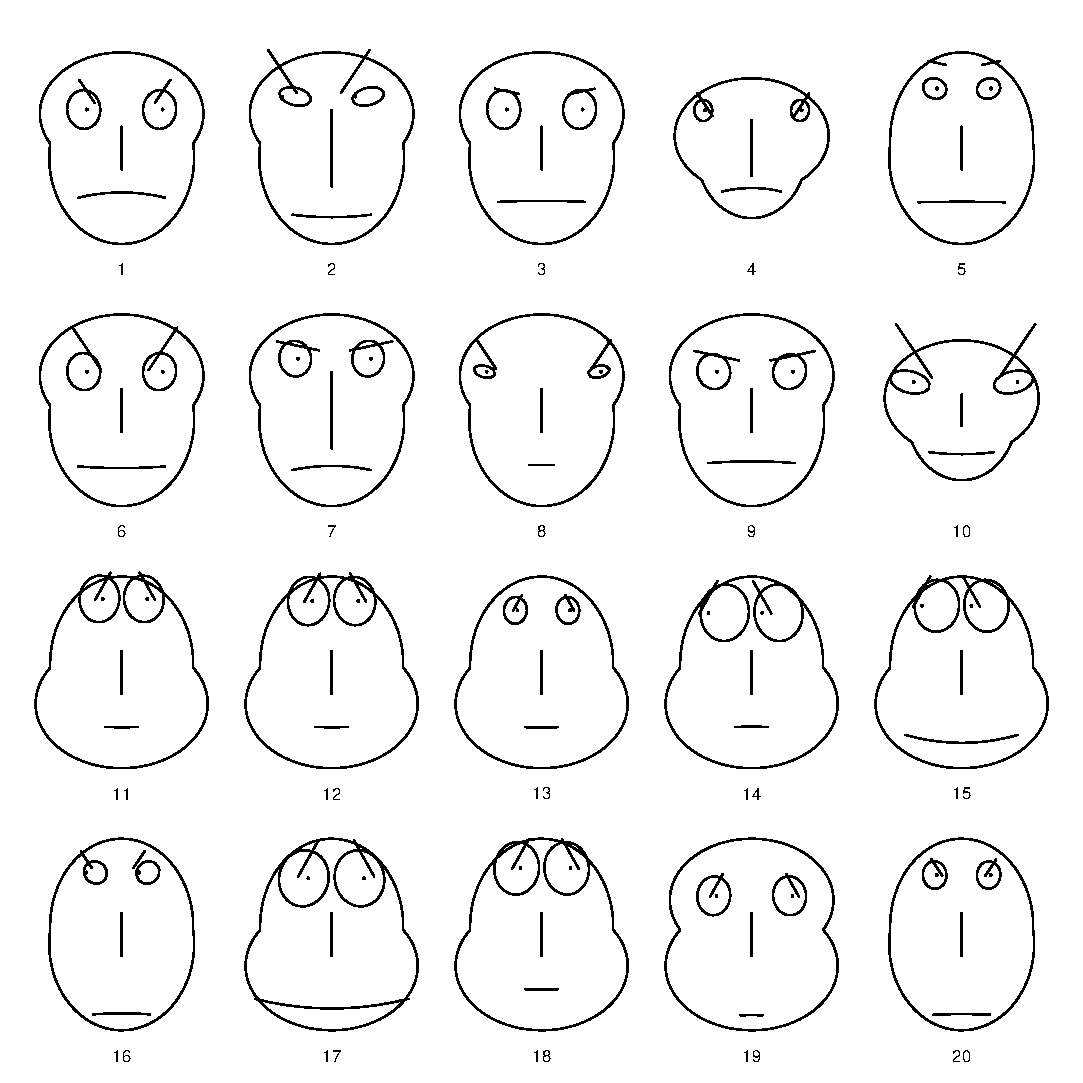
\includegraphics[height=14cm,keepaspectratio=true]{faces3.eps}
\caption{Multivariate Representation of the Utah Parolee Data}
\end{center}
\end{figure}

Although the faces do not yield perfectly uniform patterns, several distinct similarities are detectable.  The direction of the eyebrows, the width of the eyes, and the overall shape of the heads are probably the most easily recognized features that differ in a reasonably consistent manner across those who did and did not recidivate.  These features were largely determined by the employment, restitution, prior incarcerations, wage, property crime, and high school diploma variables.  A primary virtue of this graphical technique is its ability to reveal when certain types of individuals (i.e., recidivists and nonrecidivists) share many different characteristics.  Of the 10 parolees who returned to prison, 9 were unemployed, all paid restitution, 4 had committed a property crime, 3 graduated high school, and the average number of prior incarcerations was 3.6.  For the 10 parolees who did not return, 9 were employed, 2 paid restitution, none had committed a property crime, all graduated high school, and the average number of prior incarcerations was 1.4.

It is important to note that the particular type of expression conveyed by any face is meaningless.  Even though recidivists and nonrecidivists appear to communicate particular emotional states (e.g., anger, sadness, worry, etc.), these states are completely arbitrary.  By simply inverting the values of the variables or selecting different variables to assign to the facial characteristics, a recidivist could be made to express just about any emotional state.  This graphical procedure does not produce objectively meaningful emotional expressions for a given data set.  Nevertheless, the emotional expressiveness of any particular face, even when arbitrarily assigned to a random observation, does play a role in the analytical process.  The purpose of using faces for this technique is to appeal to the ability of individuals to perceive subtle differences in facial expressions in order to discern patterns in the data.    